\section{The Spectrum of Trapped Ions}
The foundation of any quantum computer is the qubits. Physical qubits can take many forms, from superconducting circuits made of Josephson junctions to topological qubits---an interesting new approach that utilizes quasiparticle excitations known as anyons. Regardless of form, our concern is with two-level quantum systems in which one state of the qubit can be readily distinguished from the other. When examining trapped ions as a candidate qubit, we have a choice on what atom and isotope we use, and the various interactions within those atoms will lead to different forms of energy level splitting in the internal electronic states \cite{Bruzewicz}. 

There are four primary domains on the spectrum of energy level splitting. Zeeman qubits (which utilize an applied field for splitting magnetic sublevels) have energy splitting on the order of tens of megahertz. Hyperfine qubits, which depend on the hyperfine energy levels of atoms arising from nucleus-electron interactions, have states separated by gigahertz, and are known for having long coherence times \cite{Warring}. Fine structure qubits, separated by tens of terahertz, display energy splitting due to the electron spin and relativistic effects. Finally, there are optical qubits whose energy levels are separated by up to hundreds of terahertz. These have properties which are advantageous to long distance entanglement mediated by photons \cite{Dietrich}.

We'll take a look at at each of these categories in more detail to discuss the mechanisms which drive them, their respective strengths and weaknesses in general, and examine their potential applications within a 2-D Coulomb crystal framework.

\begin{figure}[ht]
    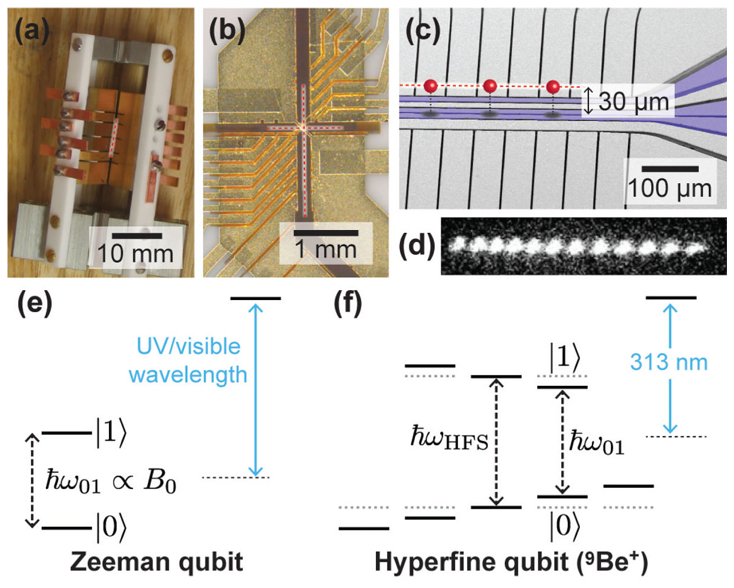
\includegraphics[width=\linewidth]{Bardin - Zeeman qubits.png}
    \caption{(\textbf{a, b}) Two types of machined 3D traps. (\textbf{c}) Schematic of a surface-electrode trap. Shown in blue are integrated microwave antenna structures that allow for qubit control. The red spheres are ions, each in its own trapping potential well. (\textbf{d}) Real image of ions in a linear trap exhibiting fluorescence due to laser excitation. (\textbf{e, f}) Energy level diagrams comparing Zeeman qubit transitions to the closely related hyperfine qubit transitions. From \textit{Microwaves in Quantum Computing} \cite{Bardin}.}
    \label{fig:Zeeman qubit}
\end{figure}

\subsection{Zeeman Qubits}
At the lower end of the energy splitting spectrum are Zeeman qubits. The isotopes chosen for this type of trapped-ion qubit are characterized as not having a nuclear spin. In this scenario, the two-level quantized states of the qubit are realized by the spin states of the ground state valence electron subject to an external magnetic field. We can do a quick calculation of the qubit resonance frequency, $\omega_{01}$, in proportion to an external magnetic field, $B_0$
\begin{equation}
    \frac{\omega_{01}}{2\pi} = \frac{\gamma_e}{2\pi}\abs{B_0}
\end{equation}
where we've used $\gamma_e/2\pi \approx$ \SI{28}{\giga\hertz\per\tesla} as the electron gyromagnetic ratio. This tells us that Zeeman qubits, with frequencies of $\sim$\SI{10}{\mega\hertz}, can be operated in magnetic fields $< \SI{1}{\milli\tesla}$. As we'll see later, hyperfine qubits can also be operated in similarly small magnetic fields (but may require larger fields for higher-mass ions). Some ions which lend themselves to acting as Zeeman qubits are \ion{174}{Yb}{+} and \ion{137}{Ba}{+} \cite{Brown, Dietrich}.

The low-frequency energy splitting, and subsequent weak magnetic field required to induce a transition, would seem to make Zeeman qubits sensitive to fluctuations in the magnetic field. That is indeed the case, and dephasing can occur for trapped ion qubits, and Zeeman qubits especially, due to deviations in the applied magnetic field. It can be shown that the first-order effects induce a shift in the frequency according to
\begin{equation}
    \Delta\nu = \frac{g_s \mu_B}{\hbar} \Delta B 
\end{equation}
where $\Delta \nu$ and $\Delta B$ are the changes in frequency and magnetic field respectively, $g_s$ is the Land\'e g-factor, $\mu_B$ is the Bohr magneton, and $\hbar$ is the reduced Planck constant. As such, magnetic field noise is a significant source of dephasing in Zeeman qubits, and the main disadvantage for using Zeeman qubits in quantum computing applications \cite{Bardin, Brown}.

However, even with that downside, Zeeman qubits offer the advantage of being resistant to leakage errors. Leakage occurs when a system contains additional states which are not used for the qubit states. Hyperfine qubits, for example, may be insensitive to first order magnetic fields, but they suffer from spontaneous scattering resulting from stimulated Raman processes that can lead to leakage (See Fig. \ref{fig:Yb qubit}). When dealing with quantum error correction, it becomes important to account for leakage out of the qubit subspace. In situations where the magnetic field can be sufficiently stabilized, $\leq$ \SI{10}{\micro\gauss}, it has been shown that Zeeman qubits exhibit a lower logical error rate when compared to similar hyperfine qubits \cite{Brown}. 

\begin{figure}[!htb]
    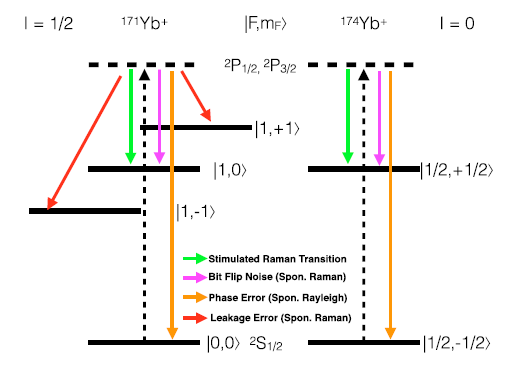
\includegraphics[width=\linewidth]{Brown - Hyperfine qubits.png}
    \caption{Energy level diagram for \ion{171}{Yb}{+} and \ion{174}{Yb}{+} ions showing the potentials errors that can occur for each scattering event. These are assuming the ion always starts in a lower qubit state. From \textit{Comparing Zeeman qubits to hyperfine qubits in the context of the surface code: \ion{174}{Yb}{+} and \ion{171}{Yb}{+}} \cite{Brown}.}
    \label{fig:Yb qubit}
\end{figure}

\subsection{Hyperfine Qubits}
Moving up the scale, we encounter hyperfine qubits, which are characterized by the interaction between their valence electron spin and nuclear spin that produces a splitting in otherwise degenerate energy levels. For example, in the \state{2}{{S}}{1/2} ground state, hyperfine splitting will produce two distinct energy levels corresponding to the difference in total angular momentum quantum number \textit{F}. 

Hyperfine qubits offer greater resistance to magnetic fields but at the cost of leakage into additional unwanted states. Similar ions can be used for hyperfine qubits as for Zeeman qubits, \ion{}{Yb}{+} being a common example, where the difference in qubit type results from the different nuclear spins amongst different isotopes. This difference in spin is due to the number of nucleons. An even number of nucleons, each with spin $1/2$, will pair off to give a total nuclear spin $I=0$. However, in isotopes with an odd number of nucleons, the unpaired nucleon contributes a spin $1/2$ so that odd-mass-number nuclei will have half-integer nuclear spin. For example, \ion{174}{Yb}{+} (used for Zeeman qubits) has a nuclear spin of $I = 0$, while \ion{171}{Yb}{+} has a nuclear spin of $I = 1/2$, making it a candidate for hyperfine qubits \cite{Brown}. 

In general, the energy level splitting for hyperfine qubits will be in the low \SI{}{\giga\hertz} range. For our example of \ion{171}{Yb}{+} the hyperfine splitting is \SI{12.6}{\giga\hertz}. The magnetic fields used to manipulate ions in this regime are still considered relatively low with $B_0 \lesssim$ \SI{50}{\milli\tesla}. Other odd isotopes that could be used for hyperfine qubits include \ion{137}{Ba}{+}, which also benefits from long-lived metastable states and the longest visible-wavelength cooling transition of any potential ionic qubit \cite{Dietrich}. In particular, there exist clock states $\ket{F=0, m_F=0}$ and $\ket{F=1, m_F=0}$ which are resistant to first-order magnetic fields. They only exhibit dependence on second-order magnetic fields, which can be derived from the Breit-Rabi formula
\begin{equation}
    \Delta \nu = \frac{(g_j - g_I)^2 \mu_B^2}{2\hbar\omega} [2B_0 \Delta B + (\Delta B)^2]
\end{equation}
where $g_J$ and $g_I$ are the electronic and nuclear Land\'e g-factors respectively, and $\omega$ is the angular frequency of the hyperfine splitting. It turns out, this second-order effect is negligibly small, so hyperfine qubits are not susceptible to magnetic field noise \cite{Brown, Bruzewicz}.

The benefits that hyperfine qubits possess don't come without their share of drawbacks. The most prominent source of errors in hyperfine qubits is population leakage outside the qubit subspace. Our idealized qubit operates as a two-level system, however, there exist additional levels in the physical system beyond the two qubit states. If the ion leaks into one of these undesirable states, that introduces errors. These types of errors are particularly harmful since standard error correction methods are not effective for treating them. There is research from Hayes \textit{et al.} that shows leakage can be suppressed by pumping from the leakage state back into the qubit state by utilizing the quadrupole transition (see Fig. \ref{fig:Leakage}) \cite{Hayes}. 
\begin{figure}[ht]
    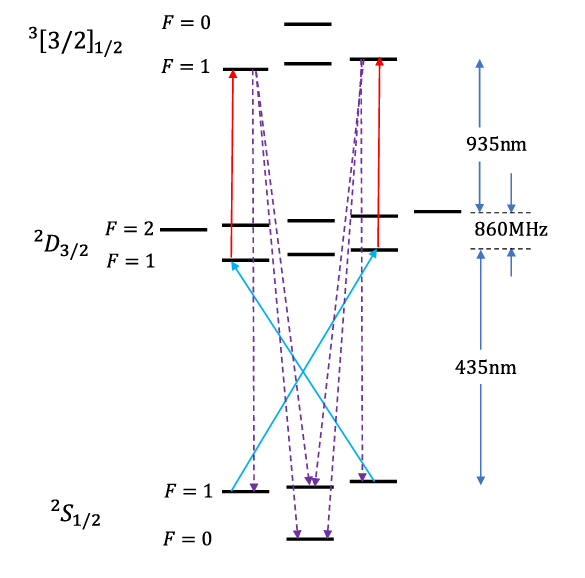
\includegraphics[width=\linewidth]{Hayes - Leakage.png}
    \caption{Energy level diagram for \ion{171}{Yb}{+}. In this repump scheme, leaked population is first driven to the \state{2}{{D}}{3/2} by the \SI{435}{\nano\meter} quadrupole transition. In the next step, the population is driven to \state{3}{[3/2]}{1/2} by the \SI{935}{\nano\meter} dipole transition. Completing the cycle, the \state{3}{[3/2]}{1/2} states decay to \state{2}{{S}}{1/2} with high probability. From \textit{Eliminating Leakage Errors in Hyperfine Qubits} \cite{Hayes}.}
    \label{fig:Leakage}
\end{figure}

\subsection{Fine Structure Qubits}
Continuing through our spectrum of trapped ion qubits, we reach fine structure qubits, which operate in the range of $\lesssim$ \SI{10}{\tera\hertz}. Similar to the hyperfine qubits we just discussed, fine structure qubits also suffer from leakage, and as a result, their lifetimes tend to be $\sim$ 1s. However, unlike hyperfine qubits, fine structure qubits fall into the category of zero nuclear spin qubits (along with Zeeman and optical qubits). As such, they typically come in the form of even mass number isotopes \cite{Bruzewicz}. An example is \ion{40}{Ca}{+} which can transition between the metastable fine structure states \state{}{D}{3/2} and \state{}{D}{5/2} that are separated by \SI{1.82}{\tera\hertz} \cite{Toyoda}. 

Stimulating these transitions for fine structure qubits is not much different from the previous qubits that we've discussed, except there are challenges that arise in generating narrow-linewidth laser beams at terahertz frequencies. One way around that is to utilize two phase-locked lasers in order to excite a stimulated Raman transition. For the \ion{40}{Ca}{+} ion, Toyoda \textit{et al.} demonstrated that phase-locked Ti:sapphire lasers at \SI{850}{\nano\meter} and \SI{854}{\nano\meter} could be used to implement a CZ gate between the qubit states $\ket{\uparrow} \equiv \ket{\text{\state{}{{D}}{5/2}} (m_J = 1/2)}$ and $\ket{\downarrow} \equiv \ket{\text{\state{}{{D}}{3/2}} (m_J = 1/2)}$ in such a way (see Fig. \ref{fig:Fine Structure}) \cite{Toyoda}. In this scheme, coherence times are potentially limited by the relative phase stability between the phase-locked laser. Nonetheless, the ease of scalability of IR lasers in integrated photonics offers a potential advantage over the blue and UV lasers required for Raman transitions in Zeeman and hyperfine qubits \cite{Bruzewicz}. 

\begin{figure}[t]
    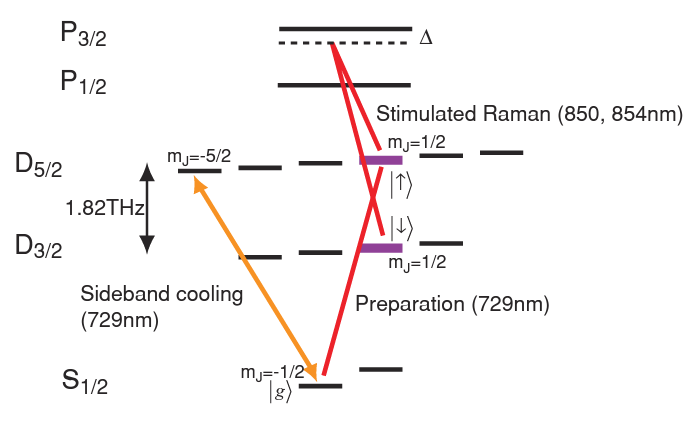
\includegraphics[width=\linewidth]{Toyoda - Fine Structure.png}
    \caption{Energy level diagram for \ion{40}{Ca}{+}. The quadrupole transition between \state{}{{S}}{1/2} and \state{}{{D}}{5/2} is used to apply a conditional phase shift while the stimulated Raman transition is used to switch between qubit states \state{}{{D}}{5/2} and \state{}{D}{3/2}, thereby implementing a CZ gate. From \textit{Quantum gate using qubit states separated by terahertz} \cite{Toyoda}.}
    \label{fig:Fine Structure}
\end{figure}

\subsection{Optical Qubits}
Finally, we reach our last stop on the energy splitting spectrum of trapped ions: optical qubits. Until now, all the previous qubit types have employed pairs of qubit states within the same orbitals. On the other hand, optical qubits generally make use of the ground-state \textit{S} level and the metastable \textit{D} level for the two qubit states. Typical energy level splitting is in the range of hundreds up to a thousand THz. 

Being optically separated allows for extremely high efficiency detection of the qubit state based on resonant fluorescence. This works by utilizing an auxiliary level which rapidly decays to the ground state. First, a laser that is resonant with the transition between the \textit{S} level ground state and the \textit{P} level auxiliary state is applied to the qubit. If the qubit is in the ground state at that time, it will be excited to the \textit{P} level, where, upon decay, it will emit a photon that can be detected. On the other hand, if the qubit is already in it's \textit{D} level upper state, then it will not be in resonance with the applied laser and the ion remains dark \cite{Bruzewicz}. 

Optical qubits are generally similar to Zeeman and fine structure qubits when it comes to choice of isotope. It's possible to base an optical qubit on odd mass number isotopes (non-zero nuclear spin) but that can lead to unwanted shifts due to hyperfine splitting in the \textit{D} state. Consequently, optical qubits will commonly make use of even mass number isotopes (zero-nuclear-spin). One such ion, \ion{88}{Sr}{+}, has been shown to be a viable candidate for optical qubits capable of implementing a universal set of gates with high fidelity. As depicted in Fig. \ref{fig:Optical}, the quantum information is encoded in states $\ket{\state{}{S}{1/2, m=+1/2}}$ and $\ket{\state{}{D}{5/2, m=+3/2}}$ \cite{Akerman}. 

This brings with it challenges related to the narrow line-widths required for the lasers used to control the optical transitions. Because fluctuations in the phase of the laser can lead to decoherence in the qubit, the lasers themselves can often become the limiting factor in coherence times \cite{Bruzewicz}. In their scheme involving the \ion{88}{Sr}{+} qubit, Akerman \textit{et al.} implemented stabilized diode lasers in a controller-follower configuration capable of producing a narrow linewidth. These diode lasers offer another advantage in that they tend to be affordable and compact compared with other light sources while still remaining capable of the precise frequencies necessary to facilitate quantum gate operations \cite{Akerman}.

Optical qubits are being studied beyond just gate operations as well. The future of fault-tolerant quantum computation is likely to rely on quantum error correction (QEC) as devices increase in scale. QEC relies on being able to detect and correct errors during computation while keeping the encoded quantum information intact and unaltered. There are various platforms, including those making use of superconducting circuits and topological features, that have been presented as possible paths to achieve this. In their 2017 paper, Bermudez \textit{et al.} examine how QEC could be implemented for trapped ions and chose to use \ion{40}{Ca}{+} ions due to the high-fidelity state detection that if offered by optical qubits (although their work shows the need for additional improvements before a truly beneficial QEC protocol can be achieved) \cite{Bermudez}.

\begin{figure}[h]
    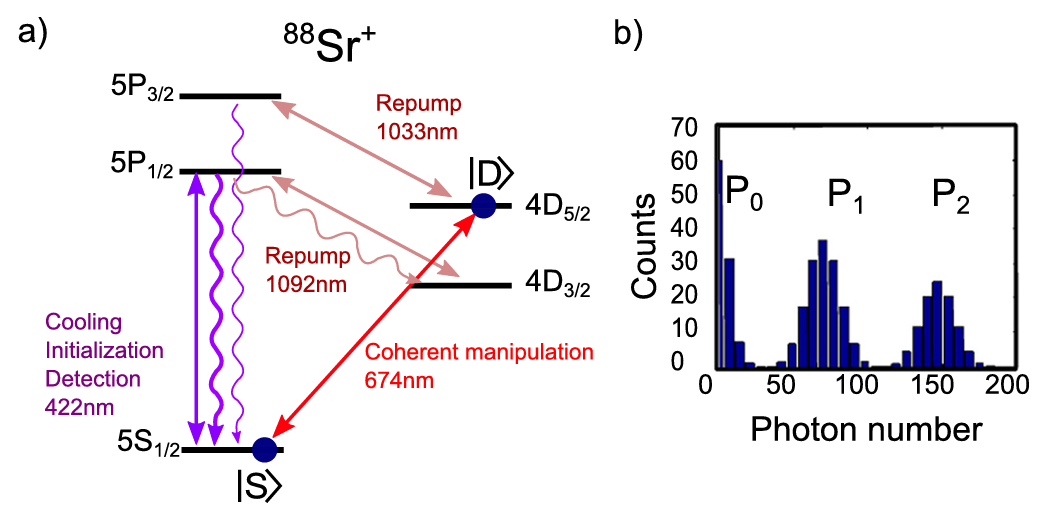
\includegraphics[width=\linewidth]{Akerman - Optical Qubits.png}
    \caption{(a) Energy level diagram for \ion{88}{Sr}{+}. The transitions depicted with straight lines are driven by lasers, while the wavy lines indicate transitions due to spontaneous emission. The thick wavy line between the \state{5}{P}{1/2} $\rightarrow$ \state{5}{S}{1/2} transition represents the fluorescence used for detection. (b) Measurements of two-qubit fluorescence. From \textit{Universal gate-set for trapped-ion qubits using a narrow linewidth diode laser} \cite{Akerman}.}
    \label{fig:Optical}
\end{figure}